\chapter{Introduction} \label{ch:introduction}

\section{Introduction}
Genetic algorithm (GA) is inspired by population genetics, and is population based, and 
proceeds over a number of generations to obtain optimal solution. GA is powerful, broadly applicable 
techniques to solve problems not yielding to other known methods. The basic mechanism of a GA, 
although there are many variants, consists of:

1. Evaluation of individual fitness and formation of a gene pool

2. Recombination and mutation.

The members of next generation population is formed by individuals produced from these operations. 
Criteria for fitness evaluation exerts evolutionary force for populations to produce more fit individuals. 
The process is repeated until system stops to improve or threshold is met.

The members of population are typically fixed length binary strings (also called genome length in later chapters). 
These members contribute to gene pool according to their relative fitness which is calculated using some objective function. 
They are mutated and recombined by crossover. Mutation corresponds to flipping the bits of an individual with some small probability, 
the mutation rate. During crossover, two parents are selected from the pool, a random but same position is chosen within 
each parent string and segments are exchanged. Small probability, crossover rate, is used perform crossover and otherwise 
parents are cloned. New offsprings produced after mutation and crossover form next generation.

Several people were working in the 1950s and the 1960s like Box (1957), Friedman (1959),
Bledsoe (1961), Bremermann (1962), and Reed, Toombs and Baricelli (1967) developed evolution-inspired algorithms 
but little attention were given to them (see \cite{Mitchell1999}). Mitchell quoted genetic algorithms were developed by Holland 
and his colleagues in the 1960s and the 1970s. Holland introduced a population-based algorithm with crossover and mutation. 
With schema theorem ( see \cite{Holland1975}), 
Holland gave some perspective on expected next generation by showing expectation of schema survival in 
next generation of population. A schema is a template that identifies a subset of strings with similarities 
at certain string positions, and a template is made up of $1$s, $0$s, and $\ast$s where 
$\ast$ is the 'don't care' symbol that matches either $0$ or $1$. However, the schema theorem by Holland 
did not compute expectation of strings in next generation which is considered of higher importance in GA. 
Bethke (see \cite{Bethke1981}) gave equations for computing expectation of number of a string in next generation. 
Goldberg (see \cite{Goldberg1987}) used equations 
for the expected next generation to model the evolutionary trajectory of a two bit GA under crossover 
and proportional selection. Vose and Liepins (see \cite{VoseLiepins1991}) simplified and extended 
these equations integrating mutation into the recombination of arbitrarily long binary strings. 
Vose and Liepins modeled simple GA by computing expected population trajectories through time based 
on infinite population. Like Goldberg, their equations are deterministic. 
Vose has proved infinite population models can be used  to explain some aspect of finite population behavior. 
Given a finite population with proportional representation vector $\bm{p}^n$ at generation $n$ with 
component $\bm{p}_i^n$ as proportion of string $i$ in finite population, infinite population model 
can be used to compute the expected proportion $\bm{p}_i^{n+1}$ of string $i$ as result of \textit{selection} and 
\textit{mixing} in next generation finite population $\bm{p}^{n+1}$.  
If $\bm{r}_{i,j}(k)$ is probability that parents $i$ and $j$ recombine to produce child $k$, and $\bm{s}_i^t$ and $\bm{s}_j^t$ 
are probability of selection of $i$ and $j$ as parents, Vose and Liepins computed expected proporiton of $k$ in next generation as
\[
\mathcal{E}(\bm{p}_k^{t+1}) = \sum_{i,j} \bm{s}_i^t \bm{s}_j^t \bm{r}_{i,j}(k) ; \text{\hspace{10pt} $\mathcal{E}$ denotes expectation}
\]
If $M$ is recombination matrix with elements $\bm{m}_{i,j} = \bm{r}_{i,j}(0)$ and permutation $\sigma_j$ defined as 
\[
\sigma_j{\langle S_0,..,S_{2^\ell - 1} \rangle}^{T} = {\langle S_{0+j},..,S_{(2^\ell - 1)+j} \rangle}^{T}
\]
where $T$ is transpose and $\ell$ is bit length of binary string, the expected proportion 
of $k$ in next generation can be represented using recombination or mixing matrix $M$ (see \cite{VoseLiepins1991}) as
\[
\mathcal{E}(\bm{p}_k^{t+1}) = (\sigma_k \bm{s})^T M (\sigma_k \bm{s})
\]
Vose and Nix (see \cite{Nix1992}) further explored issues regarding relationship between real GA and infinite population model. 
Vose and Nix obtained an exact model for real GAs in the form of a Markov chain. For a non-zero positive mutation rate, mutation 
will produce any possible string in finite population with non-zero probability and 
hence a real GA will form ergodic Markov chain, visiting every state infinitely often in a long run.
Another result Vose and Nix obtained was that trajectory followed by finite populations was related to 
the evolutionary path predicted by the infinite population model. 
Vose and Nix proved that for large populations, the evolutionary path of a real GA follows very closely, 
with large probability, and for a long period of time that path predicted by 
the infinite population model. So if we form 
a geometrical cylinder 
around the path of infinite population model, a real GA will stay inside the pipe for short term and 
then escape out of it after some period of time. 
Larger population stay inside the pipe for a longer period of time and smaller population stay inside for shorter period of time. 

% Vose and Liepins apply Walsh transform to mixing to analyse and get results. 
% With Markov chain modeling of simple GA, Vose and Nix (see \cite{Nix1992}) investigated asymptotic behavior of steady 
% state distributions as population size increases and showed that if finite population is sufficiently large, 
% convergence behavior of a real GA can be predicted. As population size increases, the correspondence improves 
% between expected population predicted using infinite population model and the actual population observed in 
% finite population genetic algorithm. 

In his book \textit{Simple Genetic Algorithm: Foundations and Theory} (see \cite{Vose1999}), Vose compiled and 
extended all of his previous work regarding infinite population model and application of walsh transforms to mixing matrix. 
Vose provided mathematical implementation of simple GA for binary strings; he provided mathematical implementation of 
selection, crossover, and mutation. Vose gave formula for calculating mixing matrix under his implementation of crossover 
and mutation. Vose discussed how application fo Walsh transform to mixing matrix simplified the matrix, giving 
computational efficiency in calculating matrix.

There had been previous applications of Walsh transform in field of GA. Bethke first introduced 
idea of using Walsh transforms to analyse process of GA in case of binary-coded strings (see \cite{Bethke1981}). The idea of using Walsh transforms 
were given greater incitement in papers by Goldberg (see \cite{Goldberg1989a}, \cite{Goldberg1989b}). But these usage of 
Walsh transforms does not involve the direct application of the Walsh transform to crossover and mutation, or to any of their 
associated mathematical objects. Vose and Liepins use Walsh transform directly to mutation and recombination, and show that the 
twist (denoted by $M_*$) of the mixing matrix ($M$) is triangularized by the Walsh transform and used $M_*$ in study of 
fixed points where $(M_*)_{i,j} = M_{i+j, i}$. In a related paper, Koehler (see \cite{Koehler1994}) gives a congruence 
transformation defined by lower triangular matrix that diagonalizes the mixing matrix for 1-point crossover and mutation 
given by a rate and mathematically proved conjecture provided by Vose and Liepins on eigenvalues of matrix $M_*$. Koehler, Bhattacharyya 
and Vose (see \cite{KoehlerBhatta1997}) applied Fourier transform to mixing in generalizing results concerning simple genetic algorithm 
which were previously established for binary case (in binary case, Fourier transform is Walsh transform) extending analysis to 
strings over an alphbet of cardinality $c$. Vose and Wright (see \cite{VoseWright1998}) applied Walsh transform to mixing matrix and 
simplified the matrix from dense to sparse in Walsh basis giving advantage of computational efficiency from 
$O(n^3)$ to $O(n^{{\log}_2 3})$. The cost of conversion of standard coordinates to Walsh basis need not be sustained 
since fast Walsh transform (see \cite{Shanks1969}) can do that in $O(n \log n)$ time.

\section{Random Heuristic Search}
Vose (see \cite{Vose1999}) introduced abstract model, a generalized heuristic search method referred 
to as {\em Random Heuristic Search (RHS)}, defined upon the central concept of state and transition 
between states. An instance of {\em RHS} is an initial collection of elements $P_0$ chosen 
from some search space $\Omega$ , together with a stochastic transition rule $\tau$ , which from $P_i$ will 
produce another collection $P_{i+1}$; iterating $\tau$ produces a sequence of generations.

The beginning collection $P_0$ is referred to as the {\em initial population}. Let $n$ be the cardinality 
of $\Omega$ and ${\bf1}$ denotes column vector of all 1s. The {\em simplex} is the set of population descriptors:

\[
\Lambda = \{x = \langle x_0,...,x_{n-1} \rangle: {\bf1}^T x=1, x_j \geq 0 \} \text{\footnotemark\label{fnm:1}}
\]
\footnotetext{$\langle .. \rangle$ represents a column vector; ${\bf1}^T$ is $\langle 1,..,1 \rangle^T$}
Element $\bm{p}$ $\in$ $\Lambda$ corresponds to a population;
$p_j$ = the proportion in the population of the $j$th element of $\Omega$.

The cardinality of each population is a constant $r$, called the population size. 
Given $r$, a population descriptor $\bm{p}$ unambiguously determines a population.

Given current population vector $\bm{p}$, the next population vector $\tau(\bm{p})$ cannot 
be predicted with certainty because $\tau$ is stochastic; it results from $r$ independent, identically distributed random choices. 
Let $\mathcal{G}:\Lambda \rightarrow \Lambda$ be a function that maps 
current population vector $\bm{p}$ to a new vector whose $i$th component 
is the probability that $i$th element of $\Omega$ is chosen. Thus, $\mathcal{G}(\bm{p})$ 
specifies the distribution from which the aggregate 
of $r$ choices forms the subsequent generation. The probability that population $\bm{q}$ is 
the next population vector given current population vector $\bm{p}$ is (see \cite{Vose1999}) 
\begin{eqnarray}
\label{Qmat}
Q_{\bm{p},\bm{q}} & = & r! \prod \frac{(\mathcal{G}(\bm{p})_j)^{r\bm{q}_j}}{(r\bm{q}_j)!} \\
 & = & \exp\{-r \sum \bm{q}_j \log \frac{\bm{q}_j}{\mathcal{G}(\bm{p})_j} - \sum (\log \sqrt{2 \pi r\bm{q}_j} \\
 + \frac{1}{12r\bm{q}_j + \theta (r\bm{q}_j)}) + O(\log r)\}
\end{eqnarray}
where summation is restricted to indices for which $\bm{q}_j > 0$.

Each random vector in the sequence $\bm{p}, \tau(\bm{p}), \tau^2(\bm{p}),...$ depends only on the value of the preceding one, 
which is a special situation. Such a sequence forms a Markov chain with transition matrix $Q_{\bm{p},\bm{q}}$. Therefore, 
the conceptualization of RHS can be replaced by Markov chain model abstraction which makes no reference to sampling $\Omega$; 
from current population $\bm{p}$, produce $\bm{q} = \tau (\bm{p})$ with probability $Q_{\bm{p},\bm{q}}$. The expected next generation 
$\mathcal{E}(\tau (\bm{p}))$ is $\mathcal{G}(\bm{p})$ (see \cite{Vose1999}). The expression in (\ref{Qmat})
\[
\sum \bm{q}_j \log \frac{\bm{q}_j}{\mathcal{G}(\bm{p})!}
\]
is the {\em discrepancy} of $\bm{q}$ with respect to $\mathcal{G}(\bm{p})$. It is a measure of how far $\bm{q}$ is from the expected next population 
$\mathcal{G}(\bm{p})$. Discrepancy is nonnegative and is zero only when $\bm{q}$ is the expected next population. Hence the factor 
\[
\exp\{-r \sum \bm{q}_j \log \frac{\bm{q}_j}{\mathcal{G}(\bm{p})_j}\}
\]
in (\ref{Qmat}) indicates the probability that $\bm{q}$ is the next generation
decays exponentially, with constant $r$ , as the discrepancy between $\bm{q}$ and the
expected next population increases.
The expression 
\[
\sum (\log \sqrt{2 \pi r\bm{q}_j} + \frac{1}{12r\bm{q}_j + \theta (r\bm{q}_j)})
\]
measures the {\em dispersion} of the population vector $\bm{q}$ and the factor
\[
\exp\{- \sum (\log \sqrt{2 \pi r\bm{q}_j} + \frac{1}{12r\bm{q}_j + \theta (r\bm{q}_j)})\}
\]
indicates the probability that $\bm{q}$ is the next generation decays exponentially with increasing dispersion and 
$\theta  =  \sum \log(e^{x_j}x_j!/x_j^{x_j})$.

\begin{figure}[H]
\begin{center}
\resizebox*{6cm}{!}{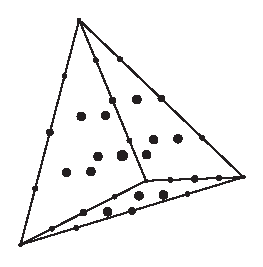
\includegraphics{figures/eps/tetra_popn.eps}}\hspace{4pt}
\caption{\textbf{Population points} }
\label{tetra_popn}
\end{center}
\end{figure}

The diagram (\ref{tetra_popn}) illustrates population points in tetrahedron for $\ell  =  2,  r  =  4$. Populations are represented by dots, 
where smaller dots have lower dispersion and larger dots have higher dispersion.

The variance of next generation population with respect to expected population (see \cite{Vose1999}) is 
\begin{equation}
\label{RHSvariance}
\mathcal{E}(\| \tau (\bm{p}) - \mathcal{G}(\bm{p}) \|^2) = (1 - \|\mathcal{G}(\bm{p})\|^2) / r
\end{equation}
It follows from Chebyshev's inequality (see \cite{ChebyshevInequality}) that 
\begin{equation}
\label{Cheby}
P(\| \tau (\bm{p}) - \mathcal{G}(\bm{p}) \| \geq \epsilon) \leq \frac{(1 - \|\mathcal{G}(\bm{p})\|^2)} {r{\epsilon}^2}
\end{equation}
where $P$ denotes probability and $\epsilon$ is arbitrary value.

Let $f(r)$ be a function which grows arbitrarily slowly, and 
\[
\lim_{r \to \infty} f(r)  =  \infty
\]
but still
\[
\lim_{r \to \infty} f(r)/\sqrt{r}  =  0.
\]
If $\epsilon  =  f(r)/\sqrt{r}$ then, (\ref{Cheby}) becomes
\begin{eqnarray*}
\lim_{r \to \infty} P(\| \tau (\bm{p}) - \mathcal{G}(\bm{p}) \| \geq \epsilon) & \leq & \frac{(1 - \|\mathcal{G}(\bm{p})\|^2)} {{f(r)}^2} \\
    & \leq & 0
\end{eqnarray*}

Therefore, $\tau(\bm{p})$ converges in probability to $\mathcal{G}(\bm{p})$ as the population size increases, 
and $\tau$ corresponds to $\mathcal{G}$ 
in the infinite population case. Moreover, (\ref{Cheby}) suggests that the distance between finite and 
infinite population in the next generation decreases as $1/\sqrt{r}$.
and mentioned $\tau (\bm{p})$ converges in probability to $\mathcal{G}(\bm{p})$ as the population size increases. 
Therefore, $\tau$ corresponds to $\mathcal{G}$ in the infinite
population case and distance between finite and infinite population in the next generation decreases as $1/\sqrt{r}$.

In the diagram (\ref{tetra_popn}), finite population points can be only at certain points, but infinite population can be anywhere on the surface. 
From theorem 3.1 in 'The Simple Genetic Algorithm: Foundations and Theory' (see \cite{Vose1999}), distance between finite population $\bm{p}$ 
and infinite population $q$ is $O(1/\sqrt{r})$. 

Let $x$ be the random variable $\| \bm{q} - \mathcal{G}(\bm{p}) \|$. Let $\phi$ be the function $\phi (x) = x^2$ 
which is convex function. Then $\mathcal{E}(\| \bm{q} - \mathcal{G}(\bm{p}) \|^2)$ becomes $\mathcal{E}(\phi (x))$. 
From Jensen's Inequality (see \cite{JensenInequality}),
if $\phi$ is a convex function, then
\begin{eqnarray*}
\phi(\mathcal{E}(x))) & \leq & \mathcal{E}(\phi(x)) \\
\mathcal{E}(x) & \leq & \sqrt{\mathcal{E}(x^2)}
\end{eqnarray*}
Substituting original variables,
\begin{equation}
\label{convergenceRHS}
\mathcal{E}(\| \bm{q} - \mathcal{G}(\bm{p}) \|) \leq \sqrt{(1 - \|\mathcal{G}(\bm{p})\|^2) / \bm{N}}
\end{equation}
Chebyshev's inequality analysis, theorem 3.1 from 'The Simple Genetic Algorithm: Foundation and Theory', 
and Jenson's inequality all points distance between finite population and infinite population is bounded 
by $1\sqrt{r}$. But it is all mathematics; what happens when real GA is run? This research explores that 
through simulations in chapter two.

An instance of RHS is called focused if $\mathcal{G}$ is continuously differentiable, and for every $\bm{p}  \in  \Lambda$
the sequence
\[
\bm{p},  \mathcal{G}(\bm{p}),  {\mathcal{G}}^2(\bm{p}),...
\]
converges. $\mathcal{G}$ is also called focused in this case and the path determined by following at each generation what $\tau$ is expected 
to produce will lead to some steady state $\omega$ such that
\[
\mathcal{G}(\omega) = \lim_n\to\infty \mathcal{G}(\bm{p}) = \omega.
\]
Such points $\omega$ are called fixed points (or limits) of $\mathcal{G}$. 
And the sequence $\bm{p},  \mathcal{G}(\bm{p}),  {\mathcal{G}}^2(\bm{p}),...$ is called orbit of $\bm{p}$ under $\mathcal{G}$. 
In case of focused $\mathcal{G}$, under some circumstances (conditions explained in chapter three), 
infinite population oscillates (see \cite{Vose1999}). If finite population converges to infinite population as population size increases, 
does it mean finite population also oscillates, if infinite population oscillates under same circumstances? 
We try to find out if finite population also oscillates with our experiment in chapter three. Then we explore 
what happens to populations if the conditions necessary for population to oscillate are violated in chapter three.





\section{Overview}
In chapter two, we describe a simple Markov model for diploid case under influence of mutation and crossover. 
The model is non-overlapping, generational, infinite population model assuming random mating and no selective pressure. 
Through abstract development, we show that the diploid model can be specialized by using mask based 
mutation and crossover operators to Vose's infinite population model which is a haploid model. Computational 
simplifications due to reduction of diploid model to haploid model and application of Walsh transform 
are exploited in experimental simulation of model, and through the experiment we demonstrate convergence 
of finite diploid population to infinite population behavior implied by equation \ref{RHSvariance}.

In chapter three, we study evolutionary limits predicted by Vose using infinite population model 
under no selective pressure. We use computation of predicted limits
of infinite population and discuss necessary and sufficient conditions stated by Vose for population
to converge in to periodic orbits. We investigate predicting the convergence of finite population 
short-term behavior to infinite population evolutionary limits under no selective pressure. 
Then it studies case of violation in the necessary and sufficient conditions for population 
to converge periodic orbits. We then study behavior of finite and infinite population when there is 
violation in necessary condition mentioned by Vose.






